\chapter{Evaluation}
%Sandra
\Autor{Sandra Schröder}\\\\
Message: In diesem Kapitel werden die beiden entwickelten Algorithmen gegenüber gestellt. Zwei zentrale Kriterien zur Evaluation der Algorithmen werden thematisiert.
\begin{itemize}
\item Skelettqualität
\item Echtzeitfähigkeit
\end{itemize}
Diese sind zentral, weil...

In den folgenden Abschnitten werden unsere Ergebnisse für die beiden Skelettierungsalgorithmen, die im
Rahmen dieser Projektarbeit entwickelt wurden, vorgestellt. Zur Bewertung der Skelettqualität greifen wir auf die
gewünschten Eigenschaften eines Skeletts zurück (Kapitel \ref{ch:Skelettierung}) und überprüfen, ob die Algorithmen sie realisieren.
\section{Skelettqualität} % message: Höhere Skelettqualität bei Thinning. Thinning-Qualität benötigt keine Verbesserungen. Aber verbesserung bei Dist. Trans. möglich.
Zum Vergleich der Algorithmen wurden Posen des Spielers aufgenommen. Bei gleichen Posen
weisen die Algorithmen deutlich unterschiedliche Resultate. Abbildung \ref{fig:vergleich-screenshot0} zeigt
den Unterkörper des Spielers. Beide Skelette beschreiben die Grundstruktur des Spieler sehr gut. Arme und Beine ... \\ Die Hände des Spielers sind deutlich vom Körper gestreckt und die Finger gespreizt. Der Thinning-Algorithmus ist in der Lage die Topologie der Hände und Finger wiederzugeben, während bei der
Distanztransformationen das Skelett der Hände gar nicht zu erkennen ist. \\
Abbildung \ref{fig:vergleich-screenshot12} zeigt ebenfalls deutliche Unterschiede in den Skeletten. Auffallend sind die Lücken in den Skelettlinien des Skeletts, das aus der Distanztransformation entstanden 
ist. Der Thinning-Algorithmus hat stets ein Skelett mit zusammenhängenden Skelettkomponenten als Ergebnis. 
Jedoch ist beim Skelett des Thinning-Algorithmus ein Ausläufer zu erkennen, der nicht die eigentliche Form
des Objektes beschreibt. Das aus der Distanztransformation resultierende Skelett gibt den Oberkörper bis
zu den Schultern als eine Linie ohne Ausläufer wieder. Wünschenswertes Ergebnis...??\\
Eine weitere Eigenschaft einer Skelettlinie ist ihre Breite, die sich idealerweise auf einen Pixel beschränkt. Dies ist beim Thinning der Fall, bei der Distanztransformation fällt die Skelettlinie breiter
aus. Wird das Skelett zur Datenkomprimierung genutzt, enthalten unnötige Pixel mehr Informationen, als 
eigentlich benötigt wird. Für andere Anwendungen muss diskutiert werden, ob...\\
Bei beiden Skeletten liegen die Skelettlinien zentriert im Objekt. 
\begin{figure}[htbp]
\centering
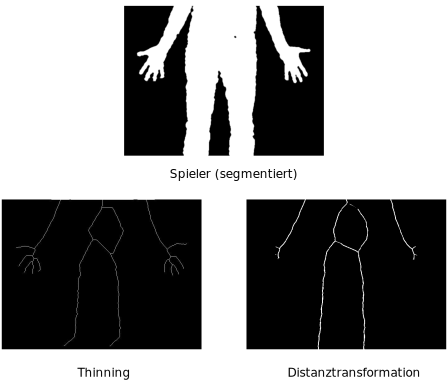
\includegraphics[width=1.0\linewidth]{./fig/vergleich-screenshot0}
\caption{}
\label{fig:vergleich-screenshot0}
\end{figure}
\begin{figure}[htbp]
\centering
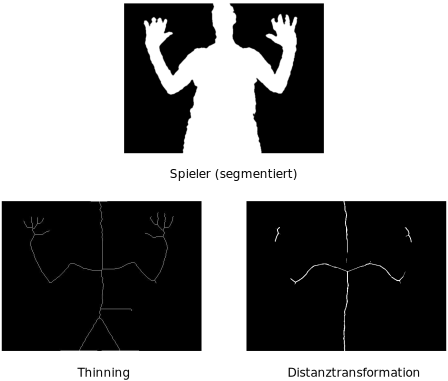
\includegraphics[width=1.0\linewidth]{./fig/vergleich-screenshot12}
\caption{}
\label{fig:vergleich-screenshot12}
\end{figure}
\clearpage
\newpage
\section{Performanz}
Die Laufzeit wurde mit dem Profiling-Tool \emph{CProfile} gemessen. Es erstellt für Python-Programme eine Statistik über die Laufzeiten eines Programms und seine einzelnen Funktionen. Es wurde jeweils eine Statistik
für die Implementierung des Thinning-Algorithmus und des Algorithmus der Distanztransformation erstellt. Die
wichtigsten Funktionen der Programme wurden aus der Statistik entnommen. Die Tabellen X und Y geben einen
Überblick über die Laufzeiten der jeweiligen Programme. \\
Obwohl der Thinning-Algorithmus bezüglich der gewünschten Eigenschaften von Skeletten die besten Ergebnisse
liefert, ist er deutlich langsamer als die Distanztransformations-Skelettierung \textbf{TODO} %TODO
\section{Verbesserung der Skelettqualität bei Dist. Trans.}
ERwähnen: Nicht während der offiziellen Projektarbeit entstanden. Es wird ein Ansatz vorgestellt.\\\\
Das Skelett, welches mit der Methode der Distanztransformation bestimmt wurde, weist Lücken zwischen den Skelettteilen auf. Um die Topologie und geometrische Eigenschaften des Objekts gut wiederzugeben, ist ein lückenloses Skelett wünschenswert. \\
Die Ursache der Lücken ist die Segmentierung des Gradientenbetrages der Distance Map. Dies wird anhand von Abbildung \ref{fig:person-skelett} deutlich. Im Gradientenbild (Teilabbildung b) sind noch durchgehende Skelettlinien zu erkennen. Per Schwellwert-Filter wird das Skelett aus dem Gradientenbild extrahiert. Für das gezeigte Beispielbild konnte allerdings kein geeigneter Schwellwert gefunden werden, der sowohl Pixelkonnektivität gewährleistet als auch Artefakte verhindert. Teilabbildung c zeight die Segmentierung des Gradientenbildes. In diesem Schritt ist die Pixelkonnektivität erstmals nicht gewährleistet. Auch in den folgenden Schritten wird die Pixelkonnektivität nicht wieder hergestellt. 
\begin{figure}[htbp]
\centering
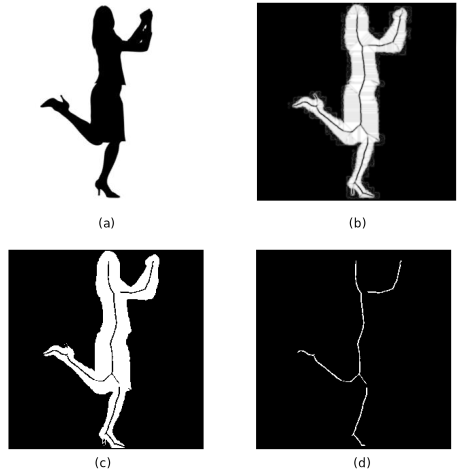
\includegraphics[width=1.0\linewidth]{./fig/person_gradienten_problem.pdf}
\caption{Bestimmung des Skelett mittels Distanztransformation. (a) Originalbild (b) Gradientenbild (c) Gradientenbild segmentiert(d) Skelett}
\label{fig:person-skelett}
\end{figure}\\
In den folgenden Abschnitten werden Methoden zur Verbesserung des Skeletts vorgestellt. Dies umfasst zum einen die Herstellung Konnektivität der Skelettkomponenten beziehungsweise dem Füllen der Lücken zwischen den Skelettlinien. Zum anderen ist es wünschenswert, dass die Skelettlinie des Objektes nicht breiter als ein Pixel ist. Zuerst wurden markante Punkte auf dem Skelett bestimmt. Diese wurden
genutzt, um mittels Breitensuche oder Tiefensuche Pfade zwischen ihnen zu finden und sie zu verbinden. Punkte werden miteinander
verbunden, wenn sie nah genug beieinander sind. Das Ergebnis ist ein Skelett mit
zusammenhängenden Skelettlinien. Die genaue Umsetzung der Algorithmen wird in den Abschnitten \ref{subsec:breitesuche} und \ref{subsec:tiefensuche} beschrieben.\\
Breiten -und Tiefensuche liefern aufgrund ihrer algorithmischen Eigenschaften jeweils unterschiedliche Ergebnisse. Die Unterschiede werden gezeigt und es wird diskutiert, inwieweit sich die Verfahren mit der Kinect anwenden lassen. 
\newpage
\subsection{Berechnung von Features auf dem Skelett}
\label{subsec:features}
Die Bildverarbeitungsbibliothek \emph{OpenCV} bietet Funktionen zur Bestimmung von markanten Punkten, sogenannten \emph{Features},
in einem Bild. Die Funktion \texttt{goodFeaturesToTrack} bestimmt die stärkesten Ecken in einem Bild oder Bildausschnitt nach einem Algorithmus von \cite{goodfeatures}. Mittels eines Qualitätsmaßes wird entschieden, ob die Stärke einer
Ecke an einem bestimmten Pixel ausreicht, um in die Featuremenge aufgenommen zu werden. Für die
Funktion können der Wert des Qualitätsmaßes, den eine Ecke erfüllen muss, die Anzahl der Ecken, die gefunden werden sollen und die
minimale Distanz zwischen den stärksten Ecken übergeben werden.\\
Die Qualität einer Ecke wird anhand von Eigenwerten bestimmt. Die Eigenwerte beziehen sich dabei auf 
die Kovarianzmatrix von Ableitungen einer festgelegten Umgebung eines Pixels. Es wird minimale Eigenwert
für die Eckendetektion weiterverwendet. Ist der minimale Eigenwert einer Ecke kleiner als das gewünschte
Qualitätsmaß, wird diese Ecke verworfen. Die verbleibenden Ecken werden nach ihrer Qualität absteigend sortiert. Anschließend wird überprüft, ob es in der spezifizierten Distanz Ecken gibt, die stärker sind. 
\begin{figure}[htbp]
\centering
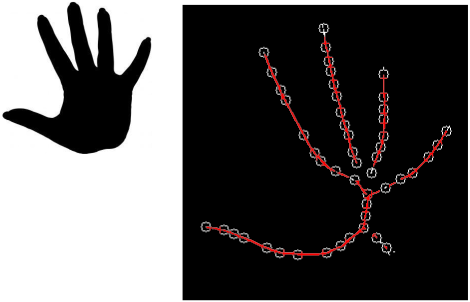
\includegraphics[width=0.4\linewidth]{./fig/features}
\caption{Ergebnis der Funktion \texttt{goodFeaturesToTrack}. Die weißen Linien markieren das Rohskelett, die Kreise markieren die Features, die auf dem Skelett gefunden wurden. Qualitätslevel: 0.1 - gewünschte Anzahl von Ecken: 50 - minimale Distanz zwischen den Ecken: 10}
\label{fig:features}
\end{figure}
Abbildung \ref{fig:features} zeigt das Ergebnis der Berechnung. Die Kreise markieren die Feature-Punkte. Wie man erkennen kann, befinden sich die Features auf der Skelettlinie. Dies ist hilfreich für die weiteren
Verbesserungen des Skeletts. Befinden sich Features außerhalb der Skelettlinien könnten die ursprüngliche Form des Skeletts und die Topologie des Objekts verfälscht werden.
\subsection{Breitensuche}
\label{subsec:breitesuche}
Der Breitensuche-Algorithmus durchsucht einen Graphen ausgehend von einem Startpunkt nach weiteren 
Knoten. Der Algorithmus sucht zunächst nur nach direkt nachfolgenden Knoten und somit in die Breite des
Graphen. Knoten, die bereits besucht wurden, werden markiert. Wurde ein Knoten noch nicht besucht, wird er
in eine \emph{Queue} (Warteschlange) aufgenommen.\\
Mittels Breitensuche sollen Pfade zwischen den markanten Punkten auf dem Skelett gefunden werden. Die markanten Punkte entsprechen Knoten in einem Graphen. Für die Nachbarschaftsbeziehung zwischen zwei
Knoten wird ein Nachbarschaftsmaß definiert. Abbildung \ref{fig:suchdistanz_naechster_nachbar} zeigt, wie überprüft wird, ob ein Punkt in einem festgelegten Intervall des Punktes $(x,y)$ liegt. Es wird eine Suchdistanz für beide Richtungen festgelegt. Sie
wird entsprechend der minimalen Distanz, die zwischen markanten Punkten erlaubt ist, gewählt (Abschnitt \ref{subsec:features}). \\
Erst wird in x-Richtung gesucht, dann in y-Richtung. Fällt der Punkt in das Intervall, wird er als besucht markiert und
mit dem Punkt $(x,y)$ verbunden. In Anhang \ref{anhang:quellcode} befindet sich der Quellcode zur Breitensuche.
%TODO: Noch weiter beschreiben: Übersicht über den Algorithmus. Bis jetzt noch ziemlich durcheinander
\begin{figure}[htbp]
\centering
\includegraphics[width=1.0\linewidth]{./fig/suchdistanz_naechster_nachbar}
\caption{Das aufgespannte Suchkreuz vom Punkt $(x,y)$ (rot) aus. Für den schwarzen Punkt wird überprüft, ob er in den festgelegten Suchintervallen des Punktes $(x,y)$ liegt.}
\label{fig:suchdistanz_naechster_nachbar}
\end{figure}\\
Das Ergebnis des Algorithmus ist in Abbildung \ref{fig:hand_BFS} im Vergleich zum vorigen Skelett zu sehen.
Das Skelett besitzt nun zusammenhängende Komponenten. Auffällig sind die Ausläufer, die auf die 
Vorgehensweise des Breitensuchealgorithmus zurückzuführen sind. Wird die Suchdistanz zu groß gewählt,
findet der Algorithmus mehrere Nachfolger, die er dann mit dem aktuellen Punkt verbindet. Das Ergebnis
sind fächerartige Ausläufer.
\begin{figure}[htbp]
	\centering
	\begin{minipage}{5cm}
		\centering
		\includegraphics[width=1.0\linewidth]{./fig/hand-skelett}
	\end{minipage}
	\hspace{2cm}
	\begin{minipage}{5cm}
		\centering
		\includegraphics[width=1.0\linewidth]{./fig/hand-bfs}
	\end{minipage}
	\caption{Ergebnis der Breitensuche.}
	\label{fig:hand_BFS}
	\end{figure}
\subsection{Tiefensuche}
\label{subsec:tiefensuche}
Wie bei der Breitensuche wird ausgehend von einem Startknoten ein Graph nach weiteren Knoten durchsucht. 
Im Gegensatz zur Breitensuche erfolgt das Traversieren des Graphens in die Tiefe. Wurde ein Nachfolgeknoten
gefunden, wird für diesen weiter geprüft, ob er ebenfalls einen Nachfolgeknoten besitzt. Dies wird
solange wiederholt (rekursiv) bis kein Nachfolgeknoten mehr gefunden werden kann. Mittels \emph{Backtracking} wird der Pfad zurückverfolgt. Anschließend wird ein neuer Knoten als Startpunkte gesucht, der noch nicht besucht wurde und das Durchsuchen nach nächsten Nachbarn wird für diesen Knoten wiederholt.\\
Die Suche nach dem nächsten Nachbarn funktioniert wie bei der Breitensuche (Abbildung \ref{fig:suchdistanz_naechster_nachbar}). Der Quellcode zum Algorithmus befindet sich im Anhang \ref{anhang:quellcode}. \\
Das Ergebnis ist in Abbildung \ref{fig:hand_DFS} zu sehen. Es fällt auf, dass es noch Lücken im Skelett gibt, was auf die Suchdistanz zurückzuführen ist. Ist sie zu klein, können keine weiteren Punkte im Umkreis des aktuellen Punktes gefunden werden und der Algorithmus endet für diesen Pfad. 
\begin{figure}[htbp]
	\centering
	\begin{minipage}{5cm}
		\centering
		\includegraphics[width=1.0\linewidth]{./fig/hand-skelett}
	\end{minipage}
	\hspace{2cm}
	\begin{minipage}{5cm}
		\centering
		\includegraphics[width=1.0\linewidth]{./fig/hand-dfs}
	\end{minipage}
	\caption{Ergebnis der Tiefensuche.}
	\label{fig:hand_DFS}
	\end{figure}\\
Das Skelett, welches aus der Tiefensuche entsteht, bedarf demnach einer Nachbearbeitung. Die Idee ist, Punkte zu finden, die keinen Nachfolger besitzen und für diese Punkte den nächsten Nachbarn zu bestimmen. Dies wird mittels eines Ansatzes realisiert, der zwischen allen Punkten ohne Nachfolger den euklidischen Abstand bestimmt und den Punkt als nächsten Nachbar wählt, der den minimalen Abstand zu dem fest gewählten Punkt hat. In Abbildung \ref{fig:hand-punkte-ohne-nachfolger} wurden die Punkte ohne Nachfolger eingezeichnet. Diese befinden sich
genau am Ende eines Pfades. Sie entsprechen den Blättern des Baumes, der bei der Tiefensuche für einen Startknoten entsteht. 
\begin{figure}[htbp]
\centering
\includegraphics[width=0.4\linewidth]{./fig/hand-DFS-ohne-nachfolger}
\caption{Punkte ohne Nachfolger nachdem das Skelett nachgezeichnet wurde (markiert mit Kreisen).}
\label{fig:hand-punkte-ohne-nachfolger}
\end{figure}
Diese Punkte wurden nun miteinander verbunden. Wie in Abbildung \ref{fig:hand-DFS-endergebnis} zu sehen ist,
wurden die Punkte ohne Nachfolger, die am nächsten beieinander sind, miteinander verbunden (rote Linien). Obwohl zwei Punkte falsche Verbindungen erzeugen, liefert der Algorithmus ein gutes Ergebnis für das Skelett. Durch Einführung weiterer Bedingungen - beispielweise, ob ein Punkt bereits verbunden ist - könnten auch diese Ausläufer eliminiert werden. 
\begin{figure}[htbp]
\centering
\includegraphics[width=0.4\linewidth]{./fig/hand-DFS-endergebnis}
\caption{Ergebnis der Tiefensuche}
\label{fig:hand-DFS-endergebnis}
\end{figure}
\section{Fazit}
1. Beide Algorithmen liefern Skelette.
2. Skelettqualität unterschiedlich. Bei Thinning hervorragend. Bei Dist.Trans. vor allem Pixelkonnektivät nicht vollständig gegeben. Es wurden Verbesserungsmöglichkeiten diskutiert, die auch zur globalen Pixelkonnektivität führen.
3. Auch mit diesen Verbessungen sollte der Dist.Trans mit etwa der vierfachen Geschwindigkeit laufen. Trotzdem mit Interpretersprache programmiert! (Im Vergleich zu Thinning.)
